%% content.tex
%%

\chapter{Status Quo}
In diesem Kapitel wollen wir den aktuellen Stand der Wissenschaft vorstellen. Hierbei beziehen wir uns auf das Thema Lernen und Online-Hilfe. Welches Wissen gibt es hierbei bereits und auf welchem Stand sind diese? Das wollen wir in diesem Kapitel klären, bevor es zu den Grundlagen dieser Arbeit kommt

\section{Lernen}
Das Thema Lernen ist ein wichtiger Bestandteil dieser Arbeit. Aus diesem Grund wollen wir uns bevor wir unsere Problemstellung einsteigen mit dem aktuellen Stand des Lernens befassen und den aktuellen Stand der Forschung zum Thema Lernen aufzeigen mit unseren in der Arbeit verwendeten Konzepten.


\subsection{Problembasiertes Lernen}
">Problem based Lerning (PBL) is a learner-centred approach for designing learning environments in authentic, ill-structured problems"< entnommen aus \cite{zumbachproblembasiertes}. \par

Das Problembasierte Lernen, wie im Zitat deutlich wird, bezieht sich auf das Erarbeiten von selbstständigen Lösungsansätzen zum Lösen eines Problems. Der Lernende soll ein Thema selbstständig erarbeiten, ohne das jemand anderes einen Lösungsweg vorzeichnet. Auf dem Weg zu der Lösung eines Problems muss er evtl. mehrere Ansätze probieren um sein Ziel zu erreichen. Wie im Zitat bereits erwähnt steht der Lernende im Mittelpunkt. Der Lernende muss hierbei selbst die Initiative ergreifen. Ein Lehrer steht beim Lernprozess nur als Helfende Hand zur Seite. Er dient dabei lediglich als Coach, der evtl. aufkommende Fragen des Lernenden beantwortet und ihn in eine spezielle Richtung leitet, falls der Lernende nicht mehr weiterkommt. Beim Thema Software haben wir eine ähnliche Problemstellung. Ein möglicher Anwender kommt an einem Punkt in der Software nicht mehr weiter und muss selbstständig eine Lösung für das konkrete Problem finden. 
 
\subsection{Differenzielles Lernen}
Ein weitere Ansatz zum Thema Lernen gibt es in der Sporttheorie. Die Idee des differenziellen Lernens bezieht sich auf das Erlernen von Bewegungen im Sport. Beim differenziellen Lernen werden Bewegungen variiert. Beim Tischtennis beispielsweise wird ein Schlag auf verschiedene Wege durchgeführt. Hierbei werden vor allem Körperwinkel variiert. \footnote{Quelle: \cite{differenziellesLernen}} Es werden drei Bälle vom Lernenden gespielt und jede Bewegung sollte hierbei auf einem anderen Weg durchgeführt werden. Das Ziel dieser Form von Lernen ist es kein ideales Technikleitbild für eine Bewegung vorzugeben, also keine Lösung sondern die Bewegung so vielfältig wie möglich zu streuen. Wenn er dieses Training durchführt, dann kann ein Lernender in jeder Situation die korrekte Bewegung anwenden. Diese Form des Bewegungslernens ist sehr stark verwandt mit dem problembasierten Ansatz. Das Differenzielle Lernen gibt ebenfalls ein Problemstellung vor, die mit verschiedenen Lösungswegen gelöst werden soll. Der Unterschied hierbei besteht in der Vorgabe von Lösungsansätzen im Vergleich zum komplett selbständigen problematisierten Lernen.  Diese beiden Konzepte des Lernens wollen wir in dieser Arbeit für unsere Empfehlung verwenden.


\chapter{Grundlagen}
Um ein besseres Verständnis dieser Arbeit zu gewährleisten, sind gewisse Grundlagen zu dem Thema erforderlich. Diese Begriffe werden nachfolgend noch einmal aufgeführt, definiert und in den Zusammenhang mit dieser Arbeit gesetzt. Beginnen möchten wir dabei mit dem Ersten der vier Begriffe, nämlich der Online-Lernhilfe.
\section{Online-Lernhilfe}
Wir werden eine kurze Begriffsdefinition geben und anschließend die Verwendung in unserer Arbeit erläutern. Dies hilft beim Verständnis des Problems.
\subsection{Begriffsdefinition}
Die Online-Lernhilfe setzt sich aus zwei Begriffen zusammen, der Online-Hilfe und der Lernhilfe. Die Online-Hilfe bezeichnet eine „\textit{Hilfefunktion, die nur über eine direkte Verbindung mit dem Internet genutzt werden kann}“ (Duden, 2015). Die Lernhilfe beschreibt eine „\textit{Hilfe, Mittel oder Anhaltspunkt beim Lernen von etwas}“ (Duden, 2015). Somit ist die Online-Lernhilfe eine Hilfe, Mittel oder Anhaltspunkt, die eine Verbindung mit dem Internet voraussetzt.

\subsection{Verwendung in der Arbeit}
Unter Online-Hilfen verstehen wir die klassischen Hilfsmodule von Software. Diese bietet dem Nutzer Hilfe zu einem bestimmten Themengebiet in der Software. Die klassische Form ist ein Handbuch das zu der Software beigelegt wird. Dieses Handbuch erklärt die Software mit ihren Funktionen. Früher waren die Handbücher sehr umfangreich, so dass man zuerst mehrere Seiten dieses Handbuch lesen musste, um die Software überhaupt erst verstehen zu können. Heutzutage sind die Benutzeroberflächen vereinfacht, so dass die Software im Idealfall selbsterklärend ist und keine weitere Hilfestellung notwendig. Das Software immer mehr Prozesse abbilden kann, wird die Komplexität einer Software jedoch immer zunehmen. Damit die Komplexität weiterhin von einem User bedient werden kann, muss er zum einen neue Bedienelemente einer Software lernen und zum Anderen eine schnelle Hilfe erhalten, wenn er an einem bestimmten Punkt in der Software nicht weiterkommt.

\section{Adaption}
\label{ch:Content1}
Wie aus dem Titel unserer Arbeit ersichtlich, benötigen wir eine Definition des Adaptions-Begriffs.

\subsection{Begriffserläuterung}
Unter dem Begriff Adaption, welcher von dem lateinischen Wort „\textit{adaptare}“ stammt und „\textit{anpassen}“ bzw. „\textit{passend}“ herrichten (Duden, 2015) bedeutet, versteht man die Anpassung eines Objekts an einen Zweck. 

\section{Adaption an den Nutzer}
Der Begriff der Adaption ist sehr breit auf den Bereich Online-Lernhilfe anwendbar. Eine Adaption ist deshalb an sehr vielen Stellen möglich. Aus diesem Grund wurde in Absprache mit den Betreuern festgestellt, dass die Lösungsvorschläge nur eine Adaption an den Nutzer beinhalten sollen.Eine Adaption an verschiedene Endgeräte, wie Tablets, Smartphones oder Computer sollen deshalb aus der Betrachtung und Bewertung ausgeschlossen werden. Lösungsvorschläge, welche im Verlauf der Arbeit vorgestellt werden und adaptiv sind, stellen folglich ausschließlich eine Anpassung an den Nutzer dar. Darunter kann man sich zum Beispiel einen grafisch aufgearbeiteten Hilfetext für den Benutzer der Software vorstellen, der sich dynamisch an den derzeit verwendeten Teil der Software anpasst.

\section{Gamification}
Als zweite Grundlage haben wir den Ansatz Gamification. Dieser ist für unsere Erläuterung sehr wichtig und wird deshalb im Folgenden aufgeführt.
\subsection{Definition}
„\textit{Gamification ist die Übertragung von spieltypischen Elementen und Vorgängen in spielfremde Zusammenhänge mit dem Ziel der Verhaltensänderung und Motivationssteigerung bei Anwenderinnen und Anwendern. Zu den spieltypischen Elementen gehören Beschreibungen (Ziele, Beteiligte, Regeln, Möglichkeiten), Punkte, Preise und Vergleiche. Zu den spieltypischen Vorgängen zählt die Bewältigung von Aufgaben durch individuelle oder kollaborative Leistungen.}“ (Bendel, 2015)

\subsection{Verwendung in unserer Arbeit}
Da es sich bei unseren Lösungsvorschlägen hauptsächlich um verschiedene Arten von Hilfen für ein konkretes Problem handelt, verwenden wir nur einen Teil aus dem Bereich des Gamification in unseren Lösungsvorschlägen. Es handelt sich bei dem verwendeten Teil um die spieltypischen Elemente, wie Punkte, Preise und Vergleiche und die spieltypischen Vorgänge. Wie diese dann konkret in unseren Lösungsvorschlägen verwendet werden, lässt sich im Kapitel der Lern-App nachlesen.

\section{Recommendersysteme}

\subsection{Begriffserläuterung}
„\textit{Ein Recommendersystem sammelt Empfehlungen von Benutzern, aggregiert diese Empfehlungen und leitet sie an geeignete Adressaten weiter.}“(aus \cite{recommender})

\subsection{Verwendung in unserer Arbeit}
In unserer Arbeit wollen wir die Recommendersysteme in Form eines Expertensystems verwenden.  Der Experte kennt ein bestimmtes Gebiet der Software und generiert später die Empfehlung. Diese kann im Kontext des Lernens entweder ein Tipp zur Lösungsfindung sein oder aber auch die direkte Lösung zu einem Problem. Im Softwareumfeld kann dies besser differenziert werden. Entweder der Experte zeigt einen möglichen  Weg auf um das Problem zu beseitigen oder aber er erarbeitet mit dem Lernenden zusammen als Coach die Lösung des Problems. Diese beiden Möglichkeiten können mithilfe eines Recommendersystems begangen werden und werden in unserem dritten Lösungsansatz weiter vertieft.






%% ===========================
\chapter{Nutzer}
Da unsere Arbeit die Adaption auf den Nutzer bezieht, müssen wir zuerst klären, welcher konkrete Nutzer bei unserer Arbeit in Frage kommt. Hierzu wollen wir die einzelnen Nutzerrollen der Zielsoftware mit deren Charakteristika vorstellen.


\section{Nutzerrollen}
Das Anwendungsfeld der Software ist wie in Einleitung beschrieben eine Hochschule. Im Mittelpunkt der Anwendung steht der Student, der sozusagen der Endkunde ist. Alle Dienstleistungen, die von der Software übernommen werden sind für den Studenten. Hierbei werden verschiedene Prozesse durchlaufen, die von verschiedenen Personen während des sogenannten Studen-Lifecycles gesteuert werden. Im folgenden werden wir erklären, wie die gegebene Nutzerrolle die Zielsoftware verwendet und welche Ziele er bei der Verwendung verfolgt.
\subsection{Professoren}
Beginnen wollen wir mit der Persona Professor. Er ist für die Lerninhaltsaufbereitung des Studenten zuständig. Ein Professor hat eher weniger mit der Software zu tun, da die meiste Arbeit die Sekretärin abnimmt. Die Verwendung beschränkt sich auf das Lesen eines Termines oder das Eintragen einer Lehrveranstaltung. Weiterhin auf ein eventuelles Einladungsmanagement. Ein Professor ist somit ein Nutzer, der sehr wenig Zeit mit der Verwendung der Software aufbringt. Somit muss er, wenn er in einem Problem bei der Verwendung der Software steckt schnell eine Lösung haben. Weiterhin ist die Zeit des Professors aufgrund seiner Aufgabengebiete begrenzt, womit eine lange Einarbeitungszeit ebenfalls vermieden werden sollte.
\subsection{Studenten}
Die Studenten sind wie Eingangs erwähnt die Profiteure der Software. Dadurch, dass alle Prozesse, die von der Software abgebildet werden nur für den Studenten da sind, steht er im Fokus. Die Verwendung der Software hält sich allerdings vom zeitlichen Aufwand her im Rahmen. Er verwendet zwar viele Bereiche der Software allerdings nur sehr kurz und schnell. Sein primäres Ziel bei der Verwendung ist Ähnlich dem Professor. Er möchte schnell an Informationen kommen und sich nicht lange in eine Software einarbeiten, da er andere Inhalte für sein Studium lernen muss. Somit sollte er komplizierte Lerninhalte einfach aufbereitet bekommen, so dass er schnell ein gutes Verständnis erlangen kann.

\subsection{Studierendensekretariat}
Das Studierendensekretariat oder auch Help-Desk genannt ist für die komplette Verwaltungsarbeit eines Studenten zuständig. Die Nutzer dieser Rolle verwenden die Software im täglichen Gebrauch und dies für mehrere Stunden am Tag. Aus diesem Grund müssen sie die Software möglichste effektiv und schnell beherrschen. Komplexe Prozesse bei der Bedienung der Software muss den Arbeitern geläufig sein, um effizient arbeiten zu können. Weiterhin muss bei einem konkreten Problem beim Verwenden der Software schnell Abhilfe geschaffen werden. 
\subsection{Studiengangsbearbeiter}
Eine besondere Rolle im Lebenszyklus der Software nimmt die Rolle des Studiengangsbearbeiters ein. Dieser ist für eine

\subsection{Admins}

\section{Nutzer Klassifizierung}
\begin{figure}[ht]
\begin{center}
\includegraphics[width = 0.8\textwidth]{Nutzerrollen.png}
\caption{Nutzerrollen in Form eines Netzes dargestellt}
\label{img1:userRoles}
\end{center}
\end{figure} 
\subsection{Lösungsorientierte Nutzer}
\subsection{Powernutzer}
\subsection{Gelegenheitsnutzer}
Kurze Erklärung der Klassifizierung und Herleitung der Ziele der einzelnen Nutzer
\label{ch:Content1:sec:Section2}
%% ===========================




%% content.tex
%%

%% ==============
\chapter{Lösungsansätze}

\section{Klassische Online-Hilfe}

\section{Lernspiel-App}

\section{Expertensystem}
\label{ch:Content2}
%% ==============



\chapter{Empfehlung}

\chapter{Zusammenfassung mit Fazit}


